\documentclass{article}\usepackage[]{graphicx}\usepackage[]{color}
% maxwidth is the original width if it is less than linewidth
% otherwise use linewidth (to make sure the graphics do not exceed the margin)
\makeatletter
\def\maxwidth{ %
  \ifdim\Gin@nat@width>\linewidth
    \linewidth
  \else
    \Gin@nat@width
  \fi
}
\makeatother

\definecolor{fgcolor}{rgb}{0.345, 0.345, 0.345}
\newcommand{\hlnum}[1]{\textcolor[rgb]{0.686,0.059,0.569}{#1}}%
\newcommand{\hlstr}[1]{\textcolor[rgb]{0.192,0.494,0.8}{#1}}%
\newcommand{\hlcom}[1]{\textcolor[rgb]{0.678,0.584,0.686}{\textit{#1}}}%
\newcommand{\hlopt}[1]{\textcolor[rgb]{0,0,0}{#1}}%
\newcommand{\hlstd}[1]{\textcolor[rgb]{0.345,0.345,0.345}{#1}}%
\newcommand{\hlkwa}[1]{\textcolor[rgb]{0.161,0.373,0.58}{\textbf{#1}}}%
\newcommand{\hlkwb}[1]{\textcolor[rgb]{0.69,0.353,0.396}{#1}}%
\newcommand{\hlkwc}[1]{\textcolor[rgb]{0.333,0.667,0.333}{#1}}%
\newcommand{\hlkwd}[1]{\textcolor[rgb]{0.737,0.353,0.396}{\textbf{#1}}}%
\let\hlipl\hlkwb

\usepackage{framed}
\makeatletter
\newenvironment{kframe}{%
 \def\at@end@of@kframe{}%
 \ifinner\ifhmode%
  \def\at@end@of@kframe{\end{minipage}}%
  \begin{minipage}{\columnwidth}%
 \fi\fi%
 \def\FrameCommand##1{\hskip\@totalleftmargin \hskip-\fboxsep
 \colorbox{shadecolor}{##1}\hskip-\fboxsep
     % There is no \\@totalrightmargin, so:
     \hskip-\linewidth \hskip-\@totalleftmargin \hskip\columnwidth}%
 \MakeFramed {\advance\hsize-\width
   \@totalleftmargin\z@ \linewidth\hsize
   \@setminipage}}%
 {\par\unskip\endMakeFramed%
 \at@end@of@kframe}
\makeatother

\definecolor{shadecolor}{rgb}{.97, .97, .97}
\definecolor{messagecolor}{rgb}{0, 0, 0}
\definecolor{warningcolor}{rgb}{1, 0, 1}
\definecolor{errorcolor}{rgb}{1, 0, 0}
\newenvironment{knitrout}{}{} % an empty environment to be redefined in TeX

\usepackage{alltt}
\usepackage[sc]{mathpazo}
\renewcommand{\sfdefault}{lmss}
\renewcommand{\ttdefault}{lmtt}
\usepackage[T1]{fontenc}
\usepackage{geometry}
\geometry{verbose,tmargin=2.5cm,bmargin=2.5cm,lmargin=2.5cm,rmargin=2.5cm}
\setcounter{secnumdepth}{2}
\setcounter{tocdepth}{2}
\usepackage[unicode=true,pdfusetitle,
 bookmarks=true,bookmarksnumbered=true,bookmarksopen=true,bookmarksopenlevel=2,
 breaklinks=false,pdfborder={0 0 1},backref=false,colorlinks=false]
 {hyperref}
\hypersetup{
 pdfstartview={XYZ null null 1}}

\makeatletter
%%%%%%%%%%%%%%%%%%%%%%%%%%%%%% User specified LaTeX commands.
\renewcommand{\textfraction}{0.05}
\renewcommand{\topfraction}{0.8}
\renewcommand{\bottomfraction}{0.8}
\renewcommand{\floatpagefraction}{0.75}

\makeatother
\IfFileExists{upquote.sty}{\usepackage{upquote}}{}
\begin{document}



\title{\title{\title{\title{\title{}}}}}



\maketitle
The results below are generated from an R script.

\begin{knitrout}
\definecolor{shadecolor}{rgb}{0.969, 0.969, 0.969}\color{fgcolor}\begin{kframe}
\begin{alltt}
\hlcom{##################################}
\hlcom{# Bio 381, HW 8: Simulating Data #}
\hlcom{# 14 Mar 2022                    #}
\hlcom{# E.M. Beasley                   #}
\hlcom{##################################}

\hlkwd{library}\hlstd{(boot)}

\hlcom{# Why sim data?}
\hlcom{# Saves time- write parts of your code before you have data}
\hlcom{# Baseline for comparisons: check assumptions in your data}
\hlcom{# Test new stats techniques (this is less common)}

\hlcom{# Part 1: Normally distributed data ---------------------}
\hlcom{# Start with groups of normally distributed data}
\hlcom{# For t-tests or ANOVA}

\hlcom{# simulate groups of 20 observations}
\hlstd{group1} \hlkwb{<-} \hlkwd{rnorm}\hlstd{(}\hlkwc{n} \hlstd{=} \hlnum{20}\hlstd{,} \hlkwc{mean} \hlstd{=} \hlnum{2}\hlstd{,} \hlkwc{sd} \hlstd{=} \hlnum{1}\hlstd{)}
\hlkwd{hist}\hlstd{(group1)} \hlcom{# look at distribution}
\end{alltt}
\end{kframe}

{\centering 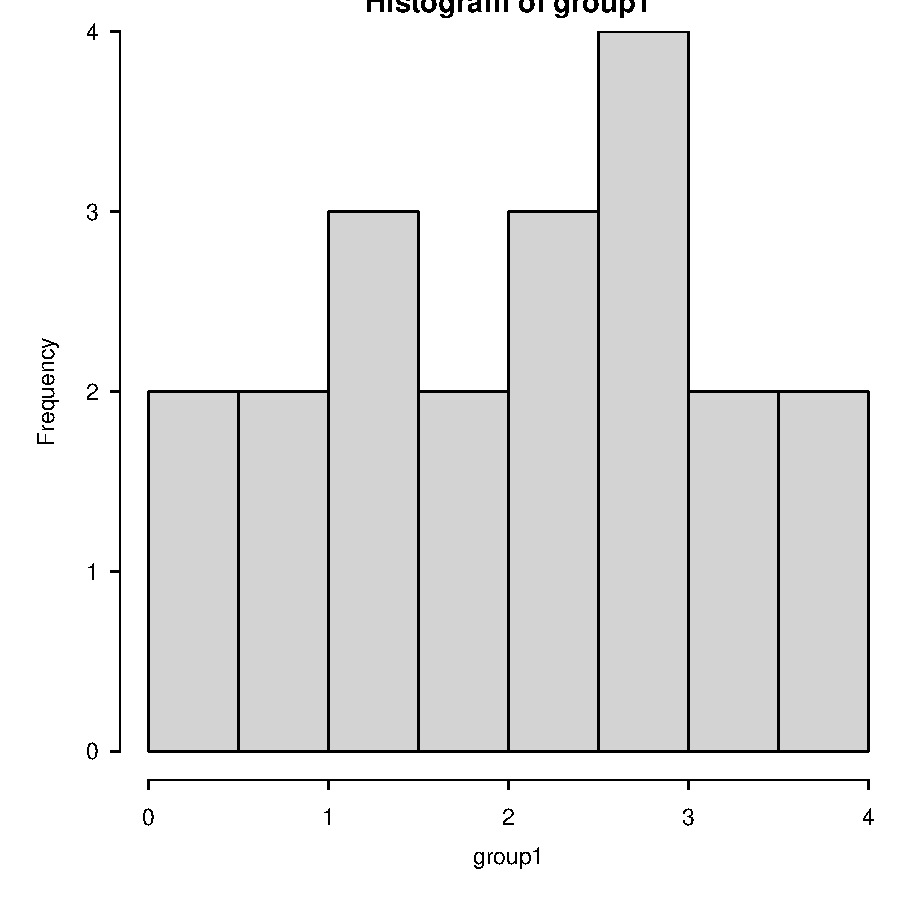
\includegraphics[width=.6\linewidth]{figure/Tutorial08-datasims-S2022-Rnwauto-report-1} 

}


\begin{kframe}\begin{alltt}
\hlcom{# change up some parameters}
\hlstd{group2} \hlkwb{<-} \hlkwd{rnorm}\hlstd{(}\hlkwc{n} \hlstd{=} \hlnum{20}\hlstd{,} \hlkwc{mean} \hlstd{=} \hlnum{5}\hlstd{,} \hlkwc{sd} \hlstd{=} \hlnum{1}\hlstd{)}
\hlstd{group3} \hlkwb{<-} \hlkwd{rnorm}\hlstd{(}\hlkwc{n} \hlstd{=} \hlnum{20}\hlstd{,} \hlkwc{mean} \hlstd{=} \hlnum{2}\hlstd{,} \hlkwc{sd} \hlstd{=} \hlnum{3}\hlstd{)}

\hlkwd{hist}\hlstd{(group2)}
\end{alltt}
\end{kframe}

{\centering 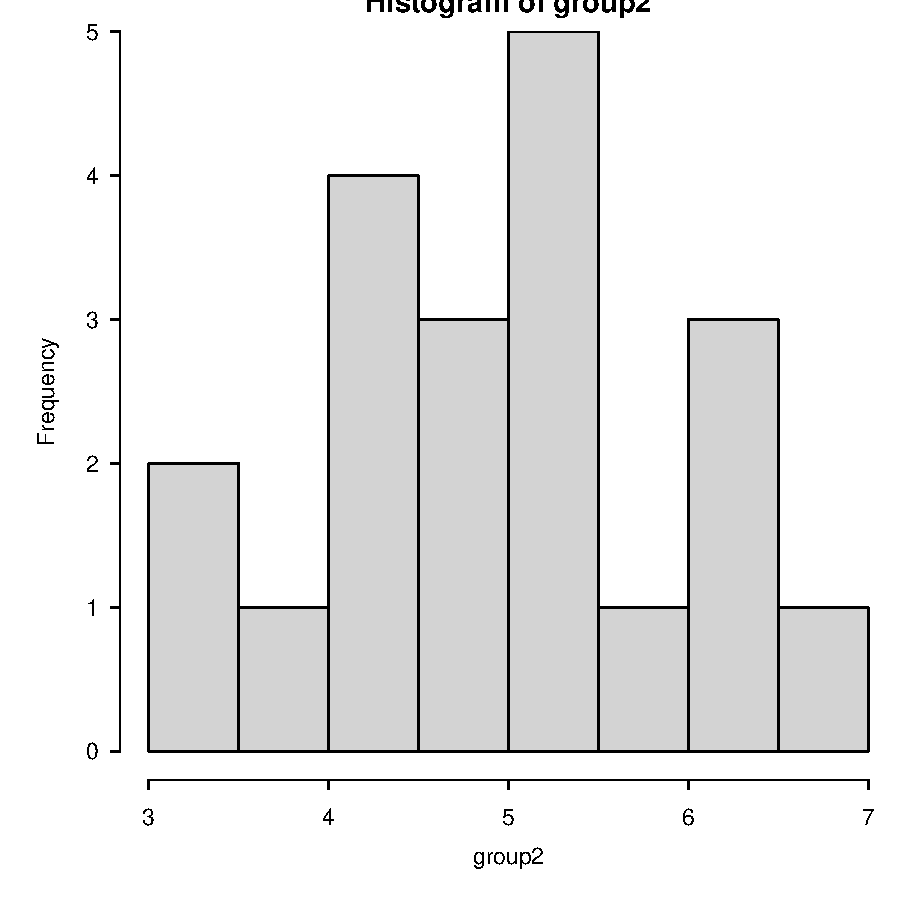
\includegraphics[width=.6\linewidth]{figure/Tutorial08-datasims-S2022-Rnwauto-report-2} 

}


\begin{kframe}\begin{alltt}
\hlkwd{hist}\hlstd{(group3)}
\end{alltt}
\end{kframe}

{\centering 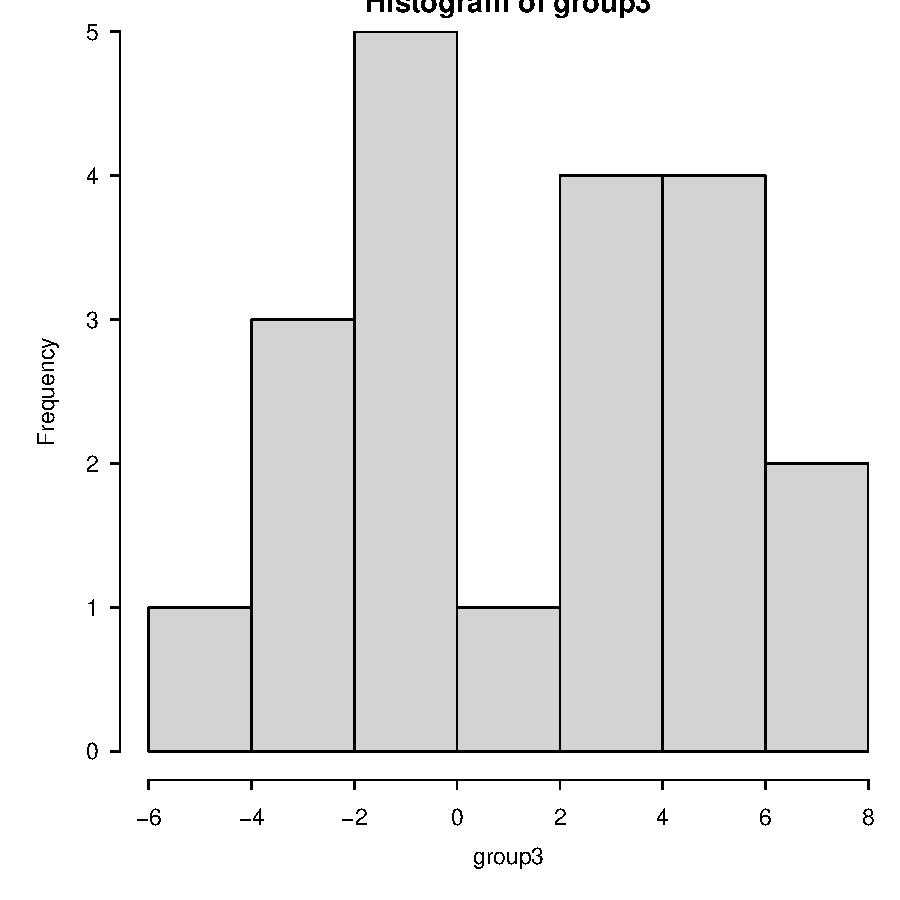
\includegraphics[width=.6\linewidth]{figure/Tutorial08-datasims-S2022-Rnwauto-report-3} 

}


\begin{kframe}\begin{alltt}
\hlcom{# You will work more with grouped data on the homework}

\hlcom{# Data sim for simple linear regression}
\hlcom{# Assume slope of 0, so y = beta1*x}
\hlcom{# where beta1 is your slope}
\hlcom{# and x is your environmental covariate}

\hlcom{# slope will be constant:}
\hlstd{beta1} \hlkwb{<-} \hlnum{1}
\hlcom{# sim the covariate:}
\hlstd{x} \hlkwb{<-} \hlkwd{rnorm}\hlstd{(}\hlkwc{n} \hlstd{=} \hlnum{20}\hlstd{)}

\hlcom{# now use the above to create a response variable:}
\hlstd{y} \hlkwb{<-} \hlstd{beta1}\hlopt{*}\hlstd{x}
\hlkwd{hist}\hlstd{(y)}
\end{alltt}
\end{kframe}

{\centering 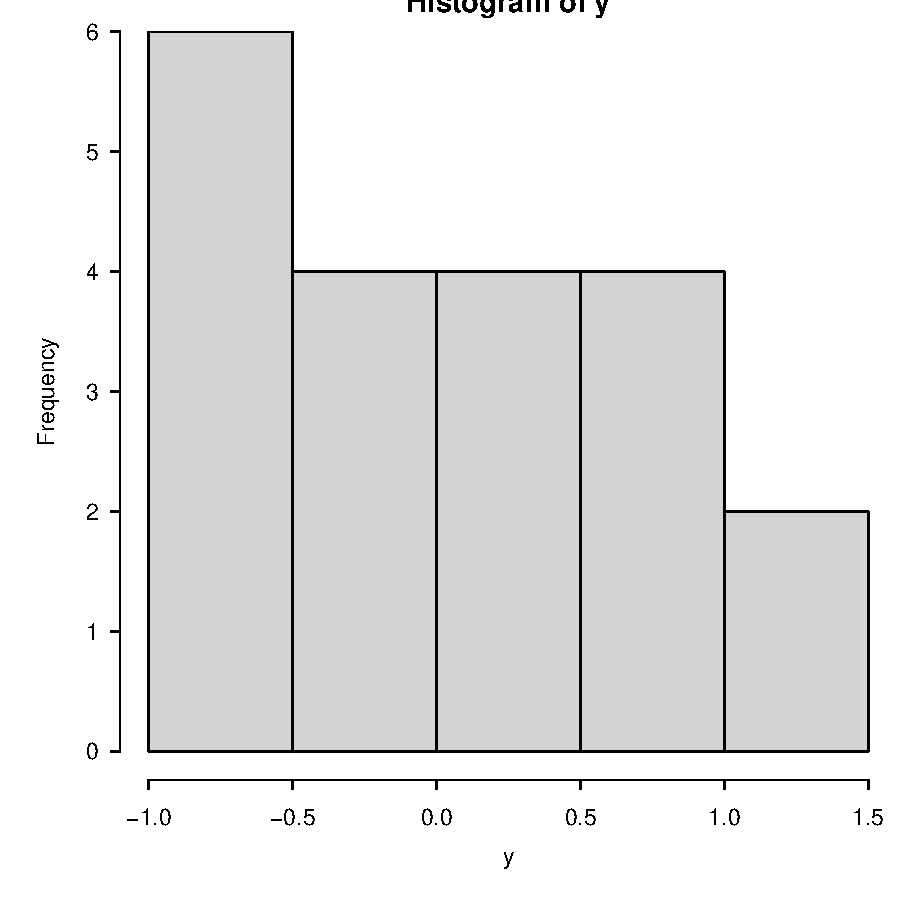
\includegraphics[width=.6\linewidth]{figure/Tutorial08-datasims-S2022-Rnwauto-report-4} 

}


\begin{kframe}\begin{alltt}
\hlcom{# you can add complexity by adding intercepts or more covariates:}
\hlstd{beta0} \hlkwb{<-} \hlnum{0.5}

\hlcom{# add intercept beta0}
\hlstd{y2} \hlkwb{<-} \hlstd{beta0} \hlopt{+} \hlstd{beta1}\hlopt{*}\hlstd{x}
\hlkwd{hist}\hlstd{(y2)}
\end{alltt}
\end{kframe}

{\centering 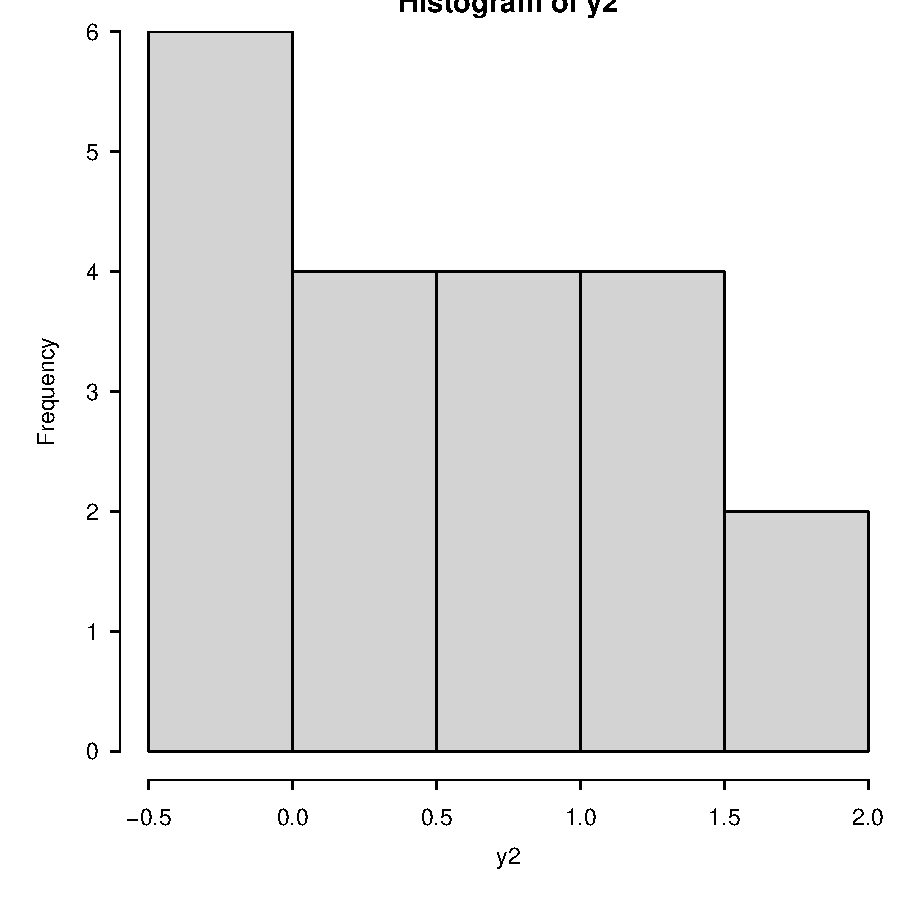
\includegraphics[width=.6\linewidth]{figure/Tutorial08-datasims-S2022-Rnwauto-report-5} 

}


\begin{kframe}\begin{alltt}
\hlcom{# You can also play with different slopes}
\hlcom{# or different distributions for the itercept/covariates}

\hlcom{# Part 2: Abundance/count data ----------------------}
\hlcom{# Option 1: data are normal-ish}
\hlcom{# use round() to get whole numbers}
\hlstd{abund1} \hlkwb{<-} \hlkwd{round}\hlstd{(}\hlkwd{rnorm}\hlstd{(}\hlkwc{n} \hlstd{=} \hlnum{20}\hlstd{,} \hlkwc{mean} \hlstd{=} \hlnum{50}\hlstd{,} \hlkwc{sd} \hlstd{=} \hlnum{10}\hlstd{))}
\hlkwd{hist}\hlstd{(abund1)}
\end{alltt}
\end{kframe}

{\centering 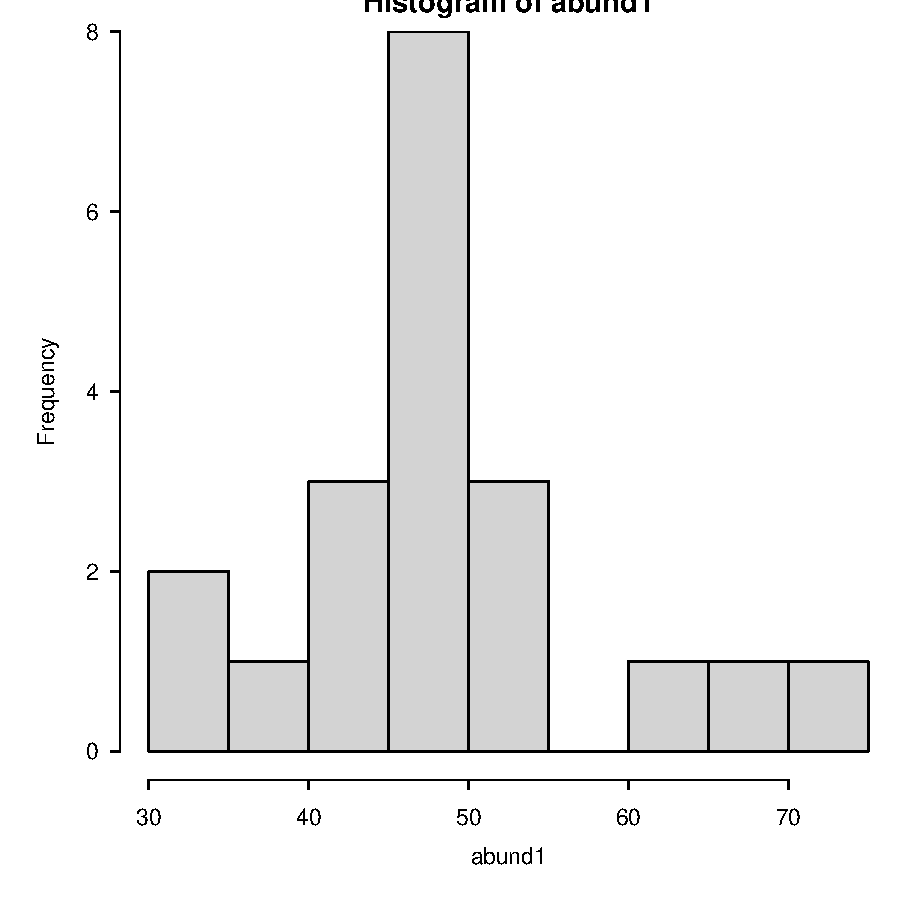
\includegraphics[width=.6\linewidth]{figure/Tutorial08-datasims-S2022-Rnwauto-report-6} 

}


\begin{kframe}\begin{alltt}
\hlcom{# this only works if sd is sufficiently large }
\hlcom{# and rnorm unlikely to get negative numbers}

\hlcom{# A better way: use Poisson distribution}
\hlcom{# Simulate counts from the same distribution}
\hlcom{# where lambda = typical abundance}
\hlstd{abund2} \hlkwb{<-} \hlkwd{rpois}\hlstd{(}\hlkwc{n} \hlstd{=} \hlnum{20}\hlstd{,} \hlkwc{lambda} \hlstd{=} \hlnum{3}\hlstd{)}
\hlkwd{barplot}\hlstd{(}\hlkwd{table}\hlstd{(abund2))}
\end{alltt}
\end{kframe}

{\centering 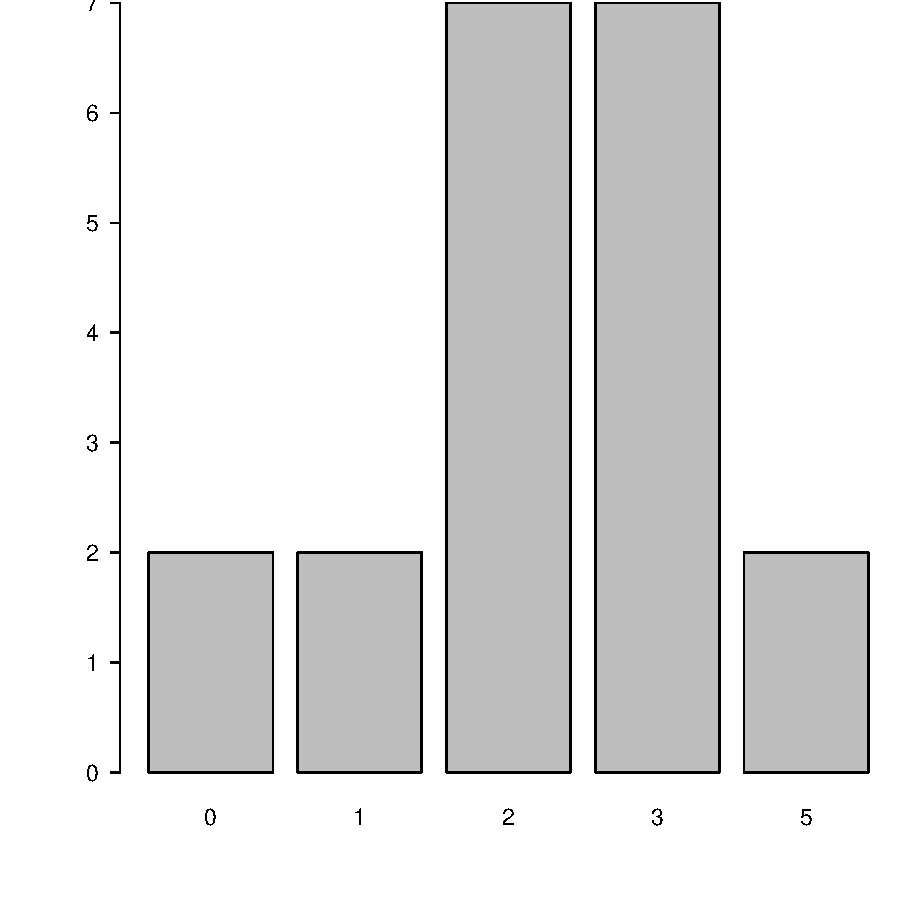
\includegraphics[width=.6\linewidth]{figure/Tutorial08-datasims-S2022-Rnwauto-report-7} 

}


\begin{kframe}\begin{alltt}
\hlcom{# Sometimes the environment affects abundance/counts}
\hlcom{# When that happens, first generate lambdas}
\hlcom{# then use those to get abundances}

\hlcom{# use regression to get initial values}
\hlstd{pre.lambda} \hlkwb{<-} \hlstd{beta0}\hlopt{+}\hlstd{beta1}\hlopt{*}\hlstd{x}
\hlcom{# use inverse log to make lambdas positive}
\hlstd{lambda} \hlkwb{<-} \hlkwd{exp}\hlstd{(pre.lambda)}

\hlcom{# use these lambda values to get abundances/counts:}
\hlstd{abund3} \hlkwb{<-} \hlkwd{rpois}\hlstd{(}\hlkwc{n} \hlstd{=} \hlnum{20}\hlstd{,} \hlkwc{lambda} \hlstd{= lambda)}
\hlkwd{hist}\hlstd{(abund3)}
\end{alltt}
\end{kframe}

{\centering 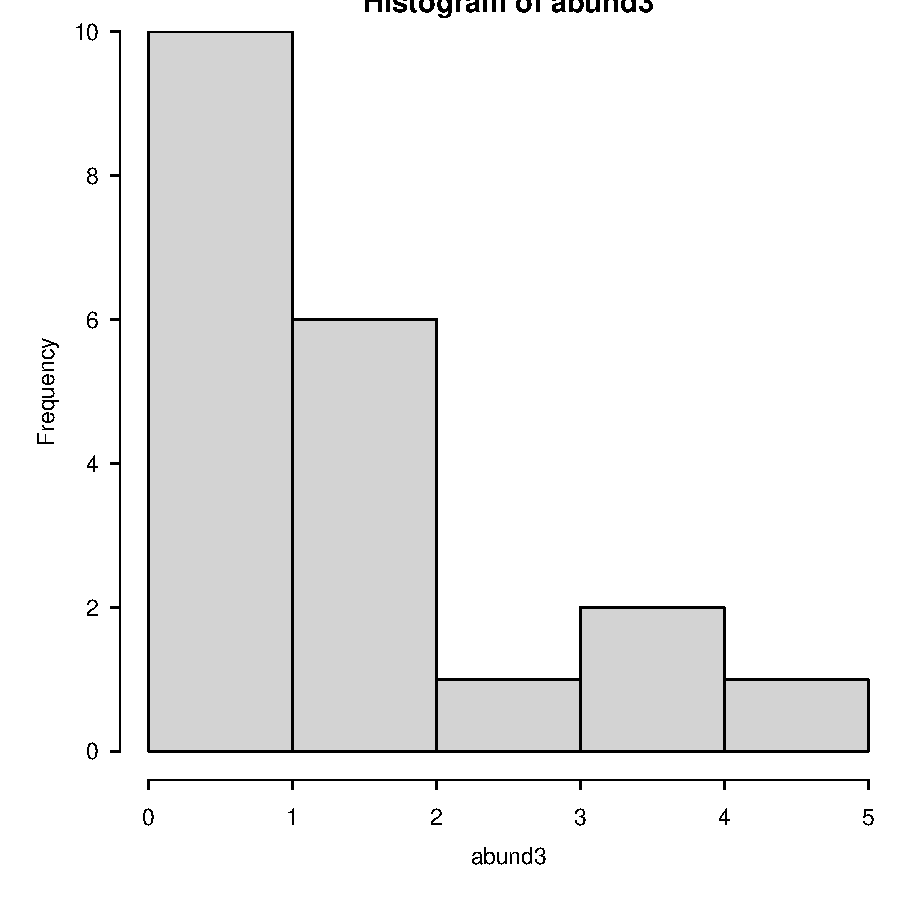
\includegraphics[width=.6\linewidth]{figure/Tutorial08-datasims-S2022-Rnwauto-report-8} 

}


\begin{kframe}\begin{alltt}
\hlcom{# Part 3: Occupancy/presence-absence data ---------------------}
\hlcom{# Option 1: getting probabilities from a beta distribution}
\hlstd{probs} \hlkwb{<-} \hlkwd{rbeta}\hlstd{(}\hlkwc{n} \hlstd{=} \hlnum{20}\hlstd{,} \hlkwc{shape1} \hlstd{=} \hlnum{1}\hlstd{,} \hlkwc{shape2} \hlstd{=} \hlnum{1}\hlstd{)}
\hlstd{occ1} \hlkwb{<-} \hlkwd{rbinom}\hlstd{(}\hlkwc{n} \hlstd{=} \hlnum{20}\hlstd{,} \hlkwc{size} \hlstd{=} \hlnum{1}\hlstd{,} \hlkwc{prob} \hlstd{= probs)}
\hlkwd{print}\hlstd{(occ1)}
\end{alltt}
\begin{verbatim}
##  [1] 0 1 0 0 0 0 0 1 1 0 0 1 1 1 0 0 0 1 0 1
\end{verbatim}
\begin{alltt}
\hlcom{# Occupancy depends on environment too}
\hlcom{# We can do something similar to above}
\hlcom{# Except we're calculating probabilities, not lambdas}

\hlstd{pre.probs} \hlkwb{<-} \hlstd{beta0} \hlopt{+} \hlstd{beta1}\hlopt{*}\hlstd{x}
\hlstd{psi} \hlkwb{<-} \hlkwd{inv.logit}\hlstd{(pre.probs)} \hlcom{# inverse logit to put on 0-1 scale}
\hlkwd{hist}\hlstd{(psi)} \hlcom{# good distribution of probs}
\end{alltt}
\end{kframe}

{\centering 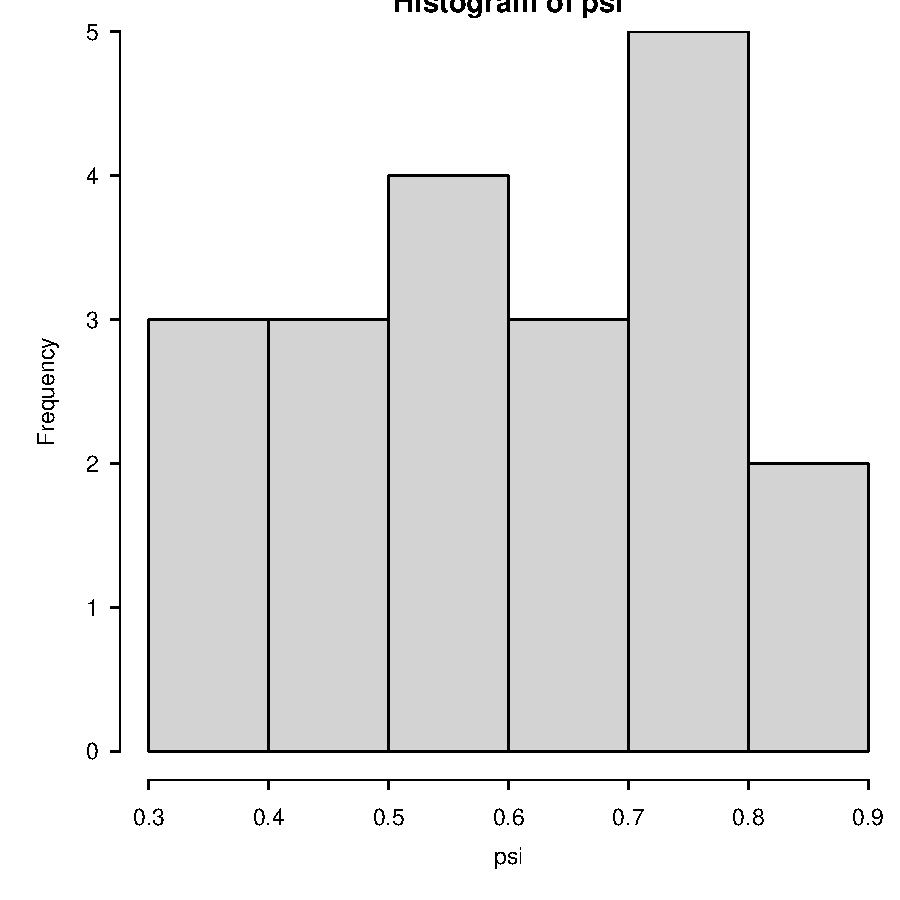
\includegraphics[width=.6\linewidth]{figure/Tutorial08-datasims-S2022-Rnwauto-report-9} 

}


\begin{kframe}\begin{alltt}
\hlcom{# use rbinom again to get occupancy data}
\hlstd{occ2} \hlkwb{<-} \hlkwd{rbinom}\hlstd{(}\hlkwc{n} \hlstd{=} \hlnum{20}\hlstd{,} \hlkwc{size} \hlstd{=} \hlnum{1}\hlstd{,} \hlkwc{prob} \hlstd{= psi)}
\hlkwd{print}\hlstd{(occ2)}
\end{alltt}
\begin{verbatim}
##  [1] 0 1 1 1 0 1 0 1 1 0 1 0 0 1 0 1 1 1 0 1
\end{verbatim}
\end{kframe}
\end{knitrout}

The R session information (including the OS info, R version and all
packages used):

\begin{knitrout}
\definecolor{shadecolor}{rgb}{0.969, 0.969, 0.969}\color{fgcolor}\begin{kframe}
\begin{alltt}
\hlkwd{sessionInfo}\hlstd{()}
\end{alltt}
\begin{verbatim}
## R version 4.1.2 (2021-11-01)
## Platform: x86_64-w64-mingw32/x64 (64-bit)
## Running under: Windows 10 x64 (build 19044)
## 
## Matrix products: default
## 
## locale:
## [1] LC_COLLATE=English_United States.1252  LC_CTYPE=English_United States.1252   
## [3] LC_MONETARY=English_United States.1252 LC_NUMERIC=C                          
## [5] LC_TIME=English_United States.1252    
## 
## attached base packages:
## [1] stats     graphics  grDevices utils     datasets  methods   base     
## 
## other attached packages:
## [1] boot_1.3-28 knitr_1.36 
## 
## loaded via a namespace (and not attached):
## [1] compiler_4.1.2 magrittr_2.0.1 tools_4.1.2    tinytex_0.35   stringi_1.7.6 
## [6] highr_0.9      stringr_1.4.0  xfun_0.27      evaluate_0.14
\end{verbatim}
\begin{alltt}
\hlkwd{Sys.time}\hlstd{()}
\end{alltt}
\begin{verbatim}
## [1] "2022-03-16 10:53:30 EDT"
\end{verbatim}
\end{kframe}
\end{knitrout}


\end{document}
